\section{Mechanika tlakové desky}

Indukčně snímaná tlaková deska funguje díky čtyřem cívkám na desce plošných spojů, které mění svojí indukčnost podle vzdálenosti snímané desky, terčíku.
Z tohoto důvodu se terčík při používání naklání, čímž zároveň mění svojí vzdálenost od jednotlivých cívek. Z toho také plyne nutnost uložit terčík
částečně volně. Terčík je proto od snímací desky oddělen pružnou vložkou, která je zároveň předepnuta pomocí nažehlovací fólie, která kryje přední 
stranu dveří a spojuje terčík s čelní krycí deskou. Díky nažehlovací fólii je také přední část dveří voděodolná.

\begin{figure}[htbp]
    \centering
    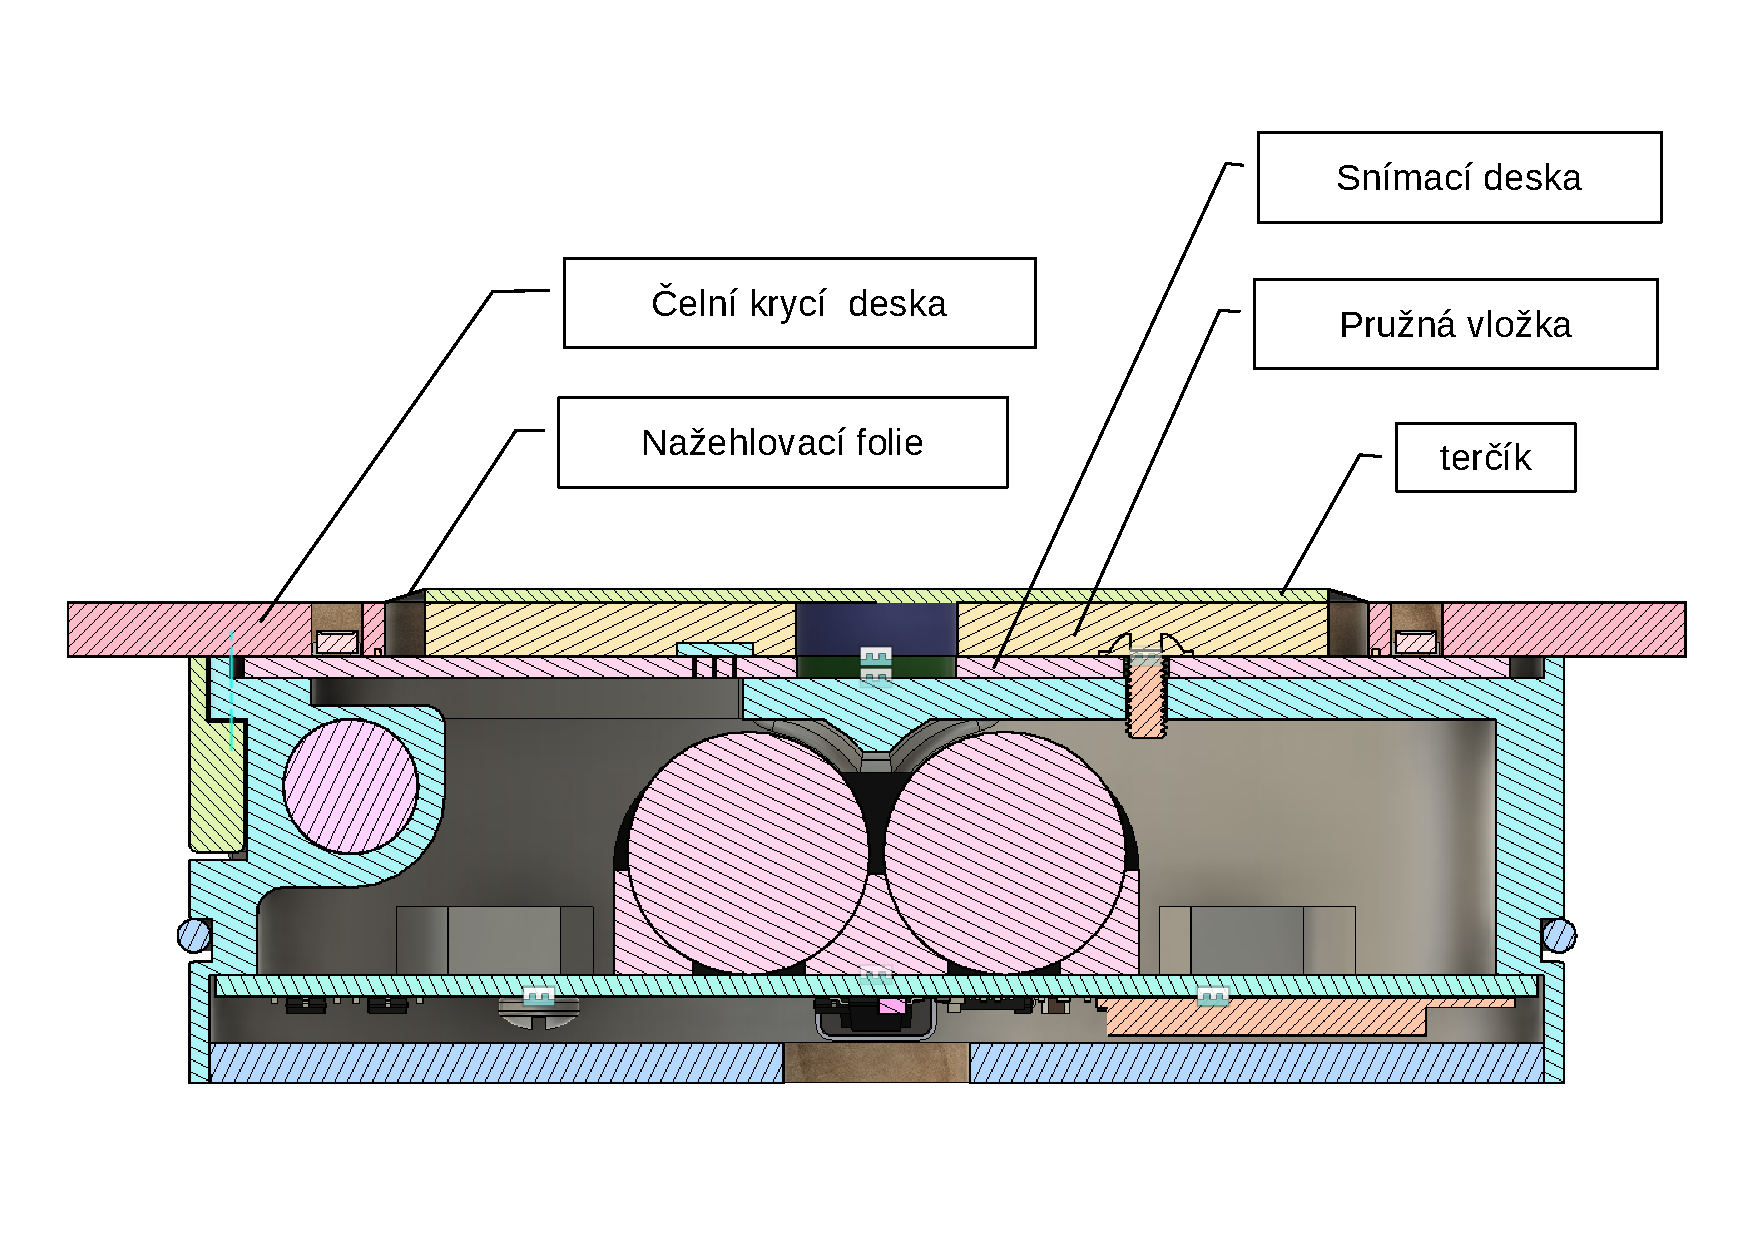
\includegraphics[width=\textwidth]{kapitoly/obrazky/E4/machanika_tlakove_desky/rez_po_ose.pdf}
    \caption{Řez varianty E4}
    \label{fig:E4-rez}
\end{figure}

Tlaková deska zárově počítá s možností působení síly o velikosti až 500~N, což samozřejmě zároveň znamená, že tělo dveří tomuto zatížení musí odolat.
Vzhledem k tomu, že nemám možnost vyrobit tělo z kovu a jsem odkázán na 3D tisk a laserovou řezačku, a zároveň chci mít dveře co možná nejmenší,
musel jsem napočítat kritické části napřesno. Z tohoto důvodu jsem v programu Fusion 360, ve kterém jsem trezor vyvíjel,
dělal simulaci, kterou zde přikládám. %todo obrázky se simulací do přílohy, a zde odkaz na č. obr a stránku, podobně i další velké obrázky (nad cca třetinu strany) 

Jako materiál těla jsem v první fázi zvolil standardní fotopolymer pro tiskárny typu SLA, s pevností v tahu 46 až 67 MPa.
V budoucnu bych ale chtěl tělo odlévat z nějakého houževnatého polyuretanu, aby se zlevnila výroba a zároveň stoupla odolnost.

\begin{figure}[htbp]
    \centering
    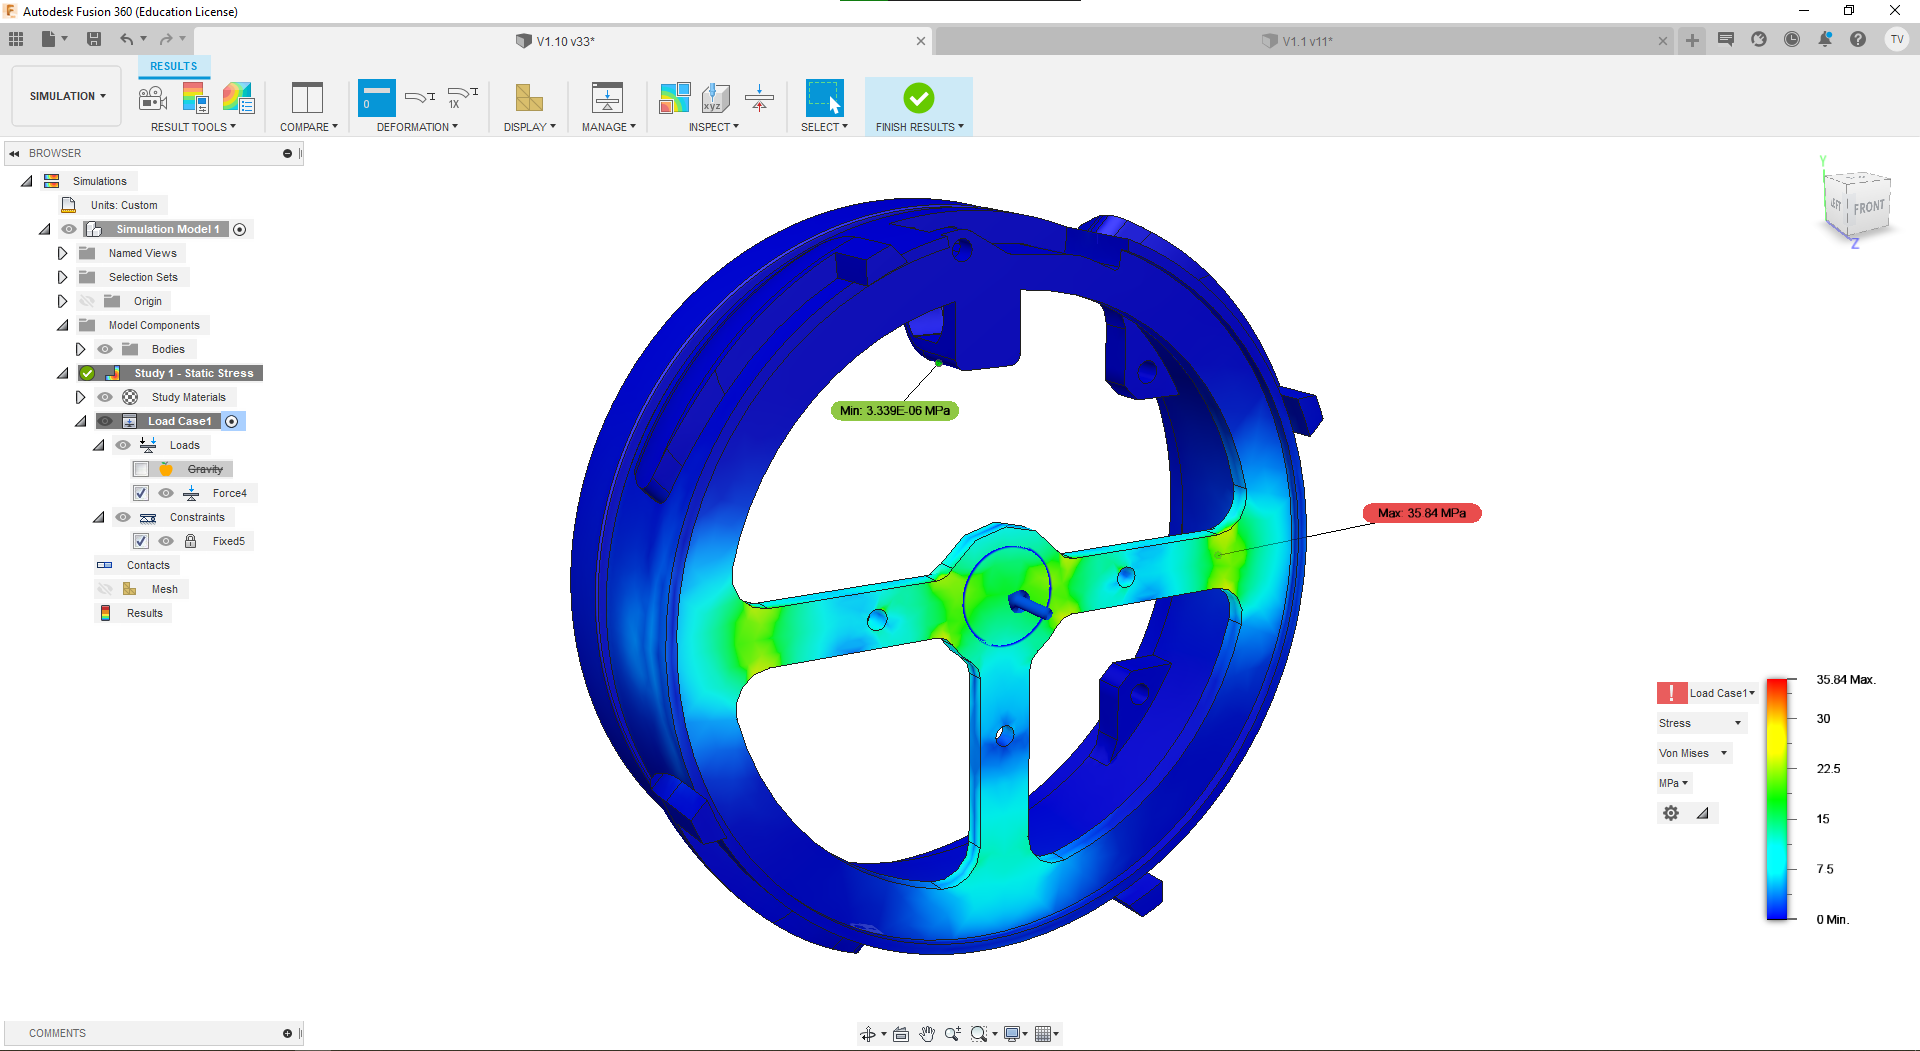
\includegraphics[width=370pt]{kapitoly/obrazky/E4/machanika_tlakove_desky/simulace/F100N,primo,uprostred,pohled_zepredu.png}
    \caption{Pevnostní simulace těla}
    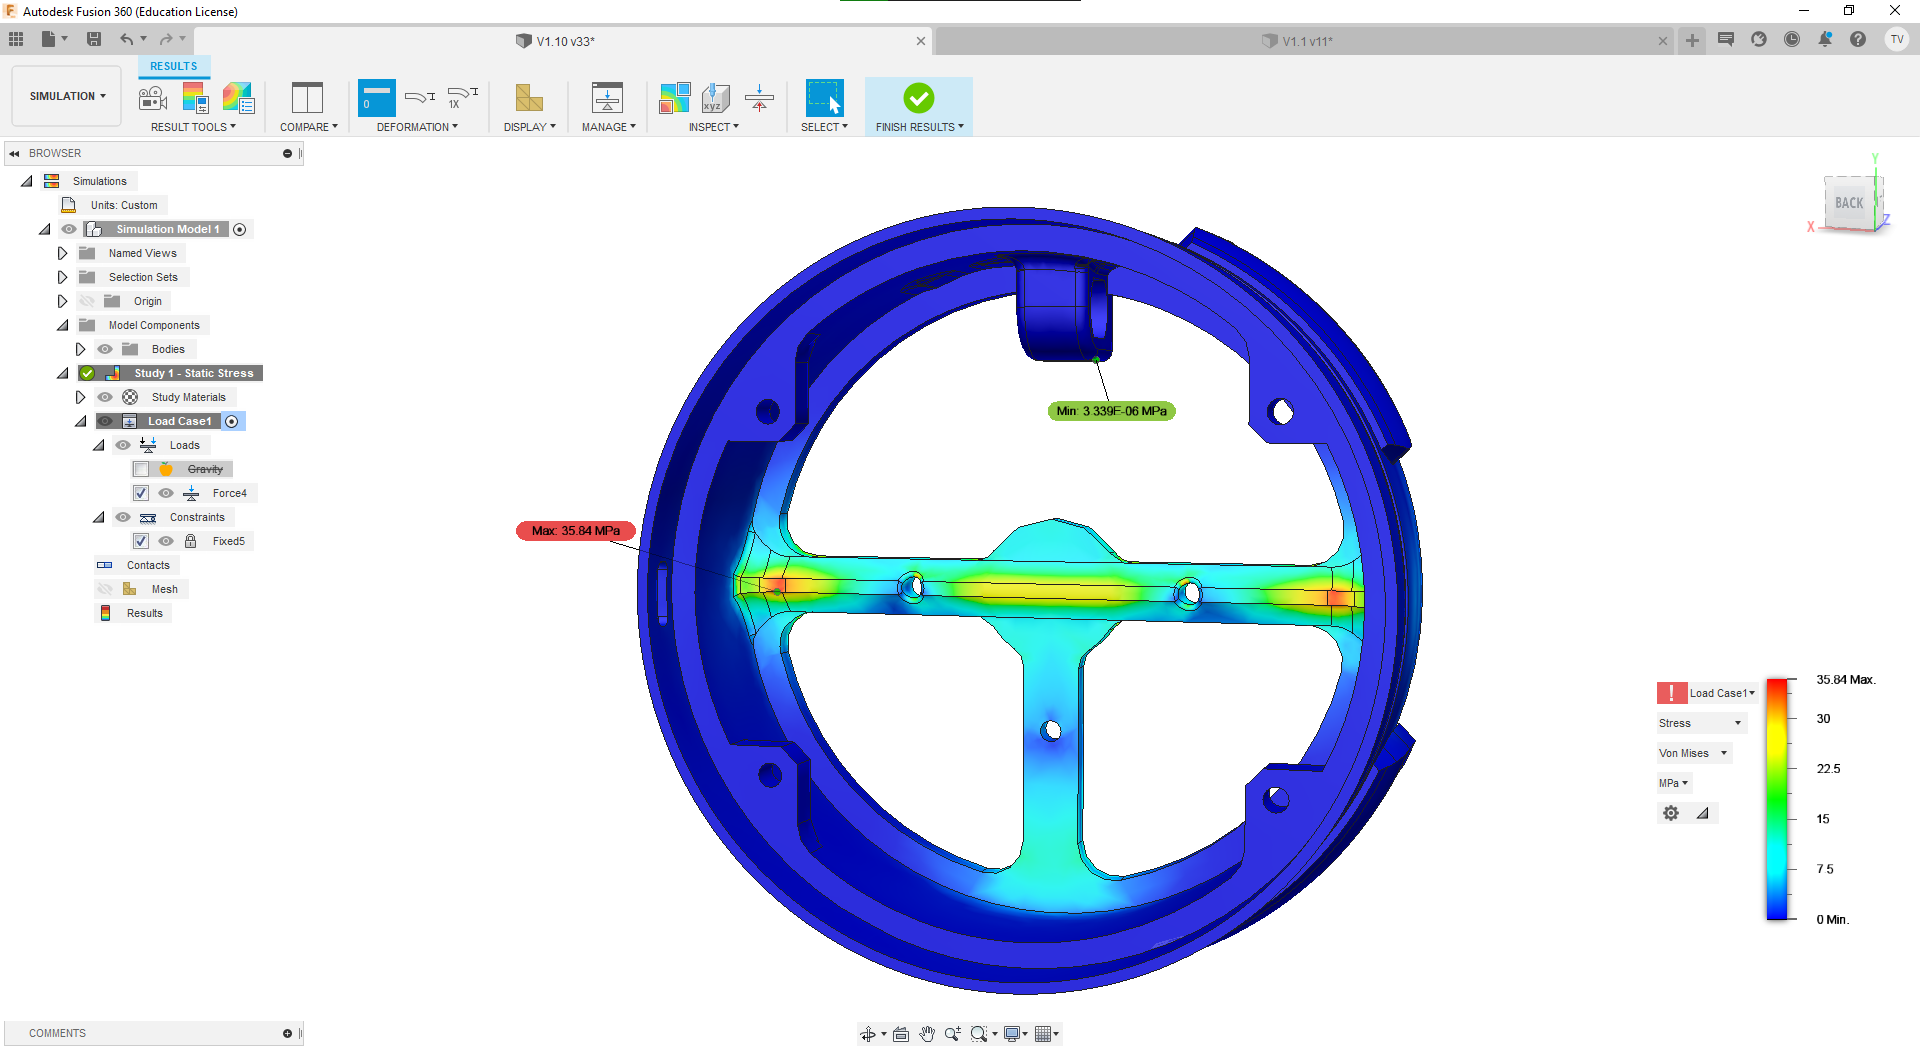
\includegraphics[width=370pt]{kapitoly/obrazky/E4/machanika_tlakove_desky/simulace/F100N,primo,uprostred,pohled_zezadu.png}
    \caption{Pevnostní simulace těla pohled zezadu}
    Tato simulace testuje působení síly přímo na tělo, což není působení, které by v provozu nastávalo. Takovéto namáhání je ale o dost náročnější
    než to, které by reálně nastalo.
    \label{fig:E4-simulace_tela} %todo těla čeho? trezor je hranatý? 
\end{figure}

\begin{figure}[htbp]
    \centering
    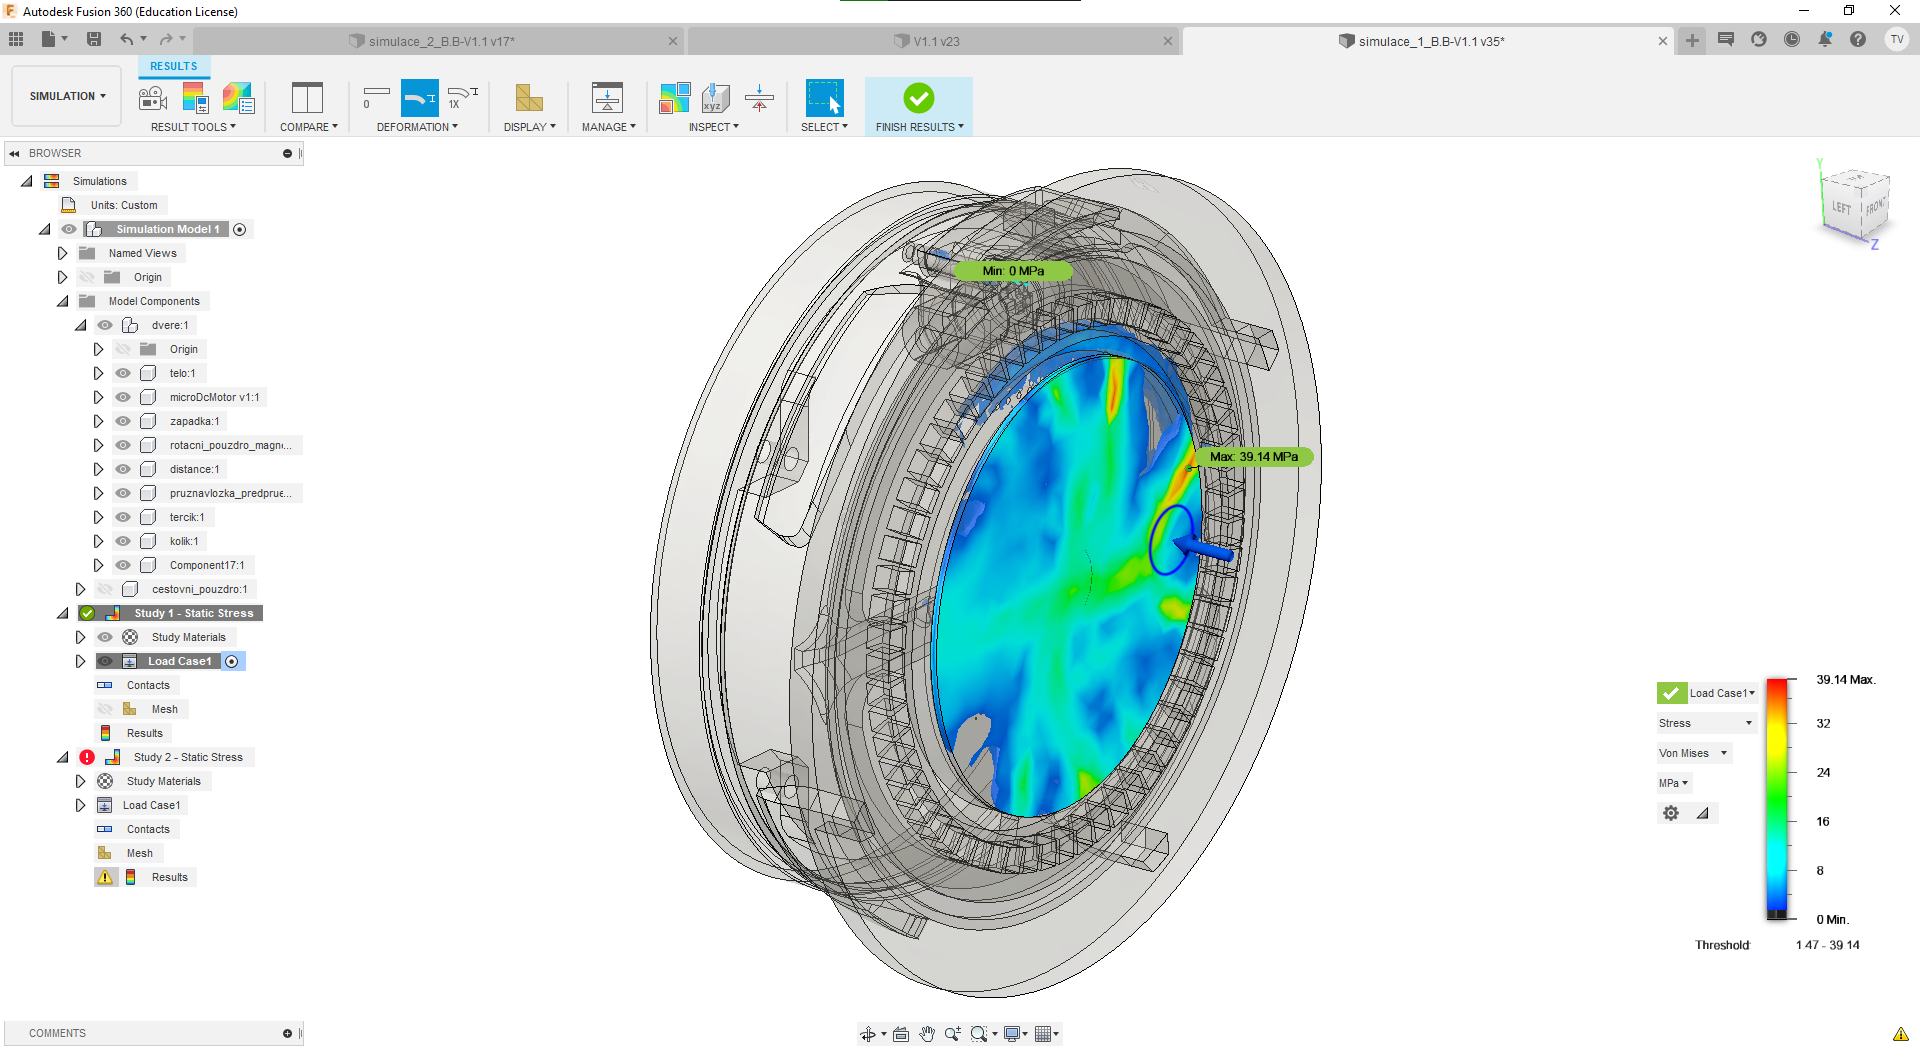
\includegraphics[width=\textwidth]{kapitoly/obrazky/E4/machanika_tlakove_desky/simulace/zjednodusena_sestava_pri_F100N_nezobrazeno_napeti_pod_1,5MPa.png}
    \caption{Simulace sestavy}
    Jak je vidět, tak i sílu 100~N dokaže sendvič z terčíku, pružné podložky a~snímací desky rozložit na dostatečnou plochu, aby napětí v těle nestouplo 
    nad cca 3~MPa. Na obrázku je zobrazené jen napětí nad 1,5~MPa.
    \label{fig:E4-simulace_tlakovky}
\end{figure}

\clearpage
\newpage